\documentclass[]{paper}
\usepackage{graphicx}
\usepackage{color}
\usepackage{fullpage}
\usepackage{subfigure}
\usepackage{url}
% type user-defined commands here
\newif\ifdraft
\drafttrue
\ifdraft
\newcommand{\onote}[1]{ {\textcolor{cyan} { (***Ole: #1) }}}
\newcommand{\terminology}[1]{ {\textcolor{red} {(Terminology used: \textbf{#1}) }}}
\newcommand{\owave}[1]{ {\cyanuwave{#1}}}
\newcommand{\jwave}[1]{ {\reduwave{#1}}}
\newcommand{\alwave}[1]{ {\blueuwave{#1}}}
\newcommand{\jhanote}[1]{ {\textcolor{red} { ***shantenu: #1 }}}
\newcommand{\alnote}[1]{ {\textcolor{green} { ***andreL: #1 }}}
\newcommand{\amnote}[1]{ {\textcolor{blue} { ***andreM: #1 }}}
\newcommand{\smnote}[1]{ {\textcolor{brown} { ***sharath: #1 }}}
\newcommand{\pmnote}[1]{ {\textcolor{brown} { ***Pradeep: #1 }}}
\newcommand{\msnote}[1]{ {\textcolor{cyan} { ***mark: #1 }}}
\newcommand{\note}[1]{ {\textcolor{magenta} { ***Note: #1 }}}
\else
\newcommand{\onote}[1]{}
\newcommand{\terminology}[1]{}
\newcommand{\owave}[1]{#1}
\newcommand{\jwave}[1]{#1}
\newcommand{\alnote}[1]{}
\newcommand{\amnote}[1]{}
\newcommand{\athotanote}[1]{}
\newcommand{\smnote}[1]{}
\newcommand{\pmnote}[1]{}
\newcommand{\jhanote}[1]{}
\newcommand{\msnote}[1]{}
\newcommand{\note}[1]{}
\fi

\begin{document}

\title{FutureGrid 2012 Project Challenge: Interoperable and
  Standards-based Distributed Cyberinfrastructure and Applications}
 
\author{Andre Luckow 
  \and Andre Merzky
  \and Mark Santcroos
  \and Ole Weidner 
  \and Shantenu Jha
}
\date{May 15th, 2012}
\maketitle

\begin{abstract}
\end{abstract}

\section{Introduction}

FutureGrid provides researchers with new possibilities to engage in
science relating to the state-of-the-art in cloud and grid
computing. As members of the RADICAL group, we have taken full
advantage of the opportunities that FutureGrid provides. Here are some
of the ways we are using FutureGrid resources to push the envelope and
pursue exciting new discoveries.

\jhanote{Topics to be covered: (i) P* (AL) (ii) CSA ? (AM) (iii)
  OGF-Standards based development and testing (AM) (iv) Class Project
  (SJ) (v) Others?}


\section{Abstraction and Runtime Environments for Distributed Cyberinfrastructure}

The seamless uptake of distributed infrastructures by scientific applications
has been limited by the lack of pervasive and simple-to-use abstractions at
multiple levels -- at the development, deployment and execution
stages~\cite{dpagrid2009}. Pilot-Jobs (PJ) provide an effective abstraction for
dynamic execution and resource utilization in a distributed context. Not
surprisingly, PJs have been one of the most successful abstractions in
distributed computing. FutureGrid has been an important resource for our
research in Pilot-based abstractions and for the development of the BigJob PJ
framework\cite{saga_bigjob_condor_cloud}.


\subsection{P* - Pilot-Job Interoperability}

Pilot-Jobs (PJ) have become one of the most successful abstractions in
distributed computing. In spite of extensive uptake, there does not
exist a well defined, unifying conceptual model of Pilot-Jobs, which
can be used to define, compare and contrast PJ implementations. This
presents a barrier to extensibility and interoperability. The P*
model~\cite{pstar-2012,pstar-sc-2012} provide a minimal but complete
model of Pilot-Jobs, which has been successfully applied to different
Pilot-Job frameworks, e.\,g.\ Condor and DIANE. The
Pilot-API~\cite{pilot_api} provides an abstract, unified interface to
PJ frameworks that adhere to the P* Model.


To demonstrated the interoperable and concurrent use of multiple Pilot-Job
frameworks via the Pilot-API on different production and research
infrastructures. For this purpose, we used BigJob as well as various other PJ 
frameworks on a heterogeneous set of infrastructure. 

Figure~\ref{fig:perf_perf-bfast-bj} shows how the Pilot-API enables the user to
run applications interoperably on different production and research
infrastructures. BigJob has been used successfully with a wide range of
applications, e.\,g.\ NAMD, Amber, Bowtie etc. For the purpose of this
investigation, we evaluate the performance of BFAST, a genome sequencing
application. For this purpose we use a problem set consisting of 
1.9\,GB reference genome and index files as well as 128 read
files (each 170\,MB). BFAST is very I/O sensitive -- we observed for example, an
I/O bottleneck if many BFAST CUs are run on the same shared file system. The
Pilot-API enables applications to scale to different infrastructures in such
cases. As shown in the figure, the FG resource was able to achieve the best 
performance.


\begin{figure}[t]
\centering
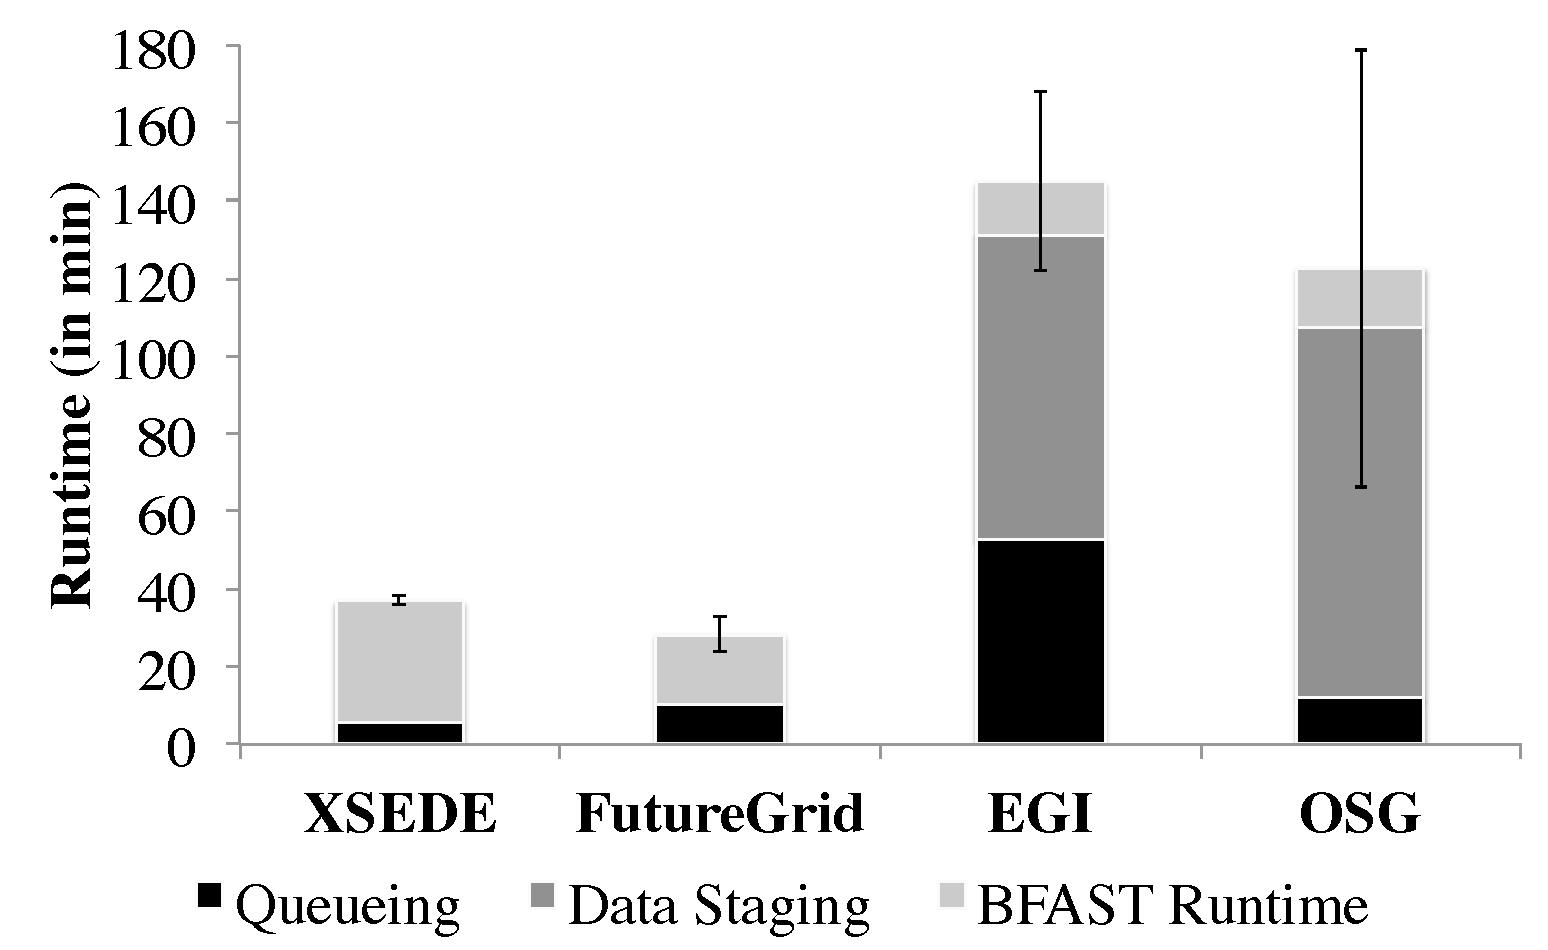
\includegraphics[width=0.7\textwidth]{figures/128-bfast-egi-fg-xsede-osg.pdf}
\caption{\textbf{PJ Framework Performance on XSEDE, FutureGrid, EGI and 
  OSG:} Running 128 BFAST match tasks on 128 cores. The longer runtimes on EGI 
  and OSG are mainly caused by  longer queuing times and the necessity to      
  stage all input files.}
  \label{fig:perf_perf-bfast-bj}
\end{figure}

\subsection{BigJob and BigData}

FutureGrid has been an important testbed for the development of
BigJob~\cite{saga_bigjob_condor_cloud} and
BigData~\cite{pstar-sc-2012,pmr-2012}. BigJob (BJ) is a SAGA-based Pilot-Job
(PJ) framework that implements the Pilot-API. BJ has been designed to be
general-purpose and extensible. While BJ has been originally built for HPC
infrastructures, such as FutureGrid and XSEDE, it is generally also usable in
other environments, such as OSG. This extensibility mainly arises from the
usage of SAGA as a common API for accessing distributed resources
interoperably (see section~\ref{sec:standards}).

\begin{figure}[t]
	\centering
	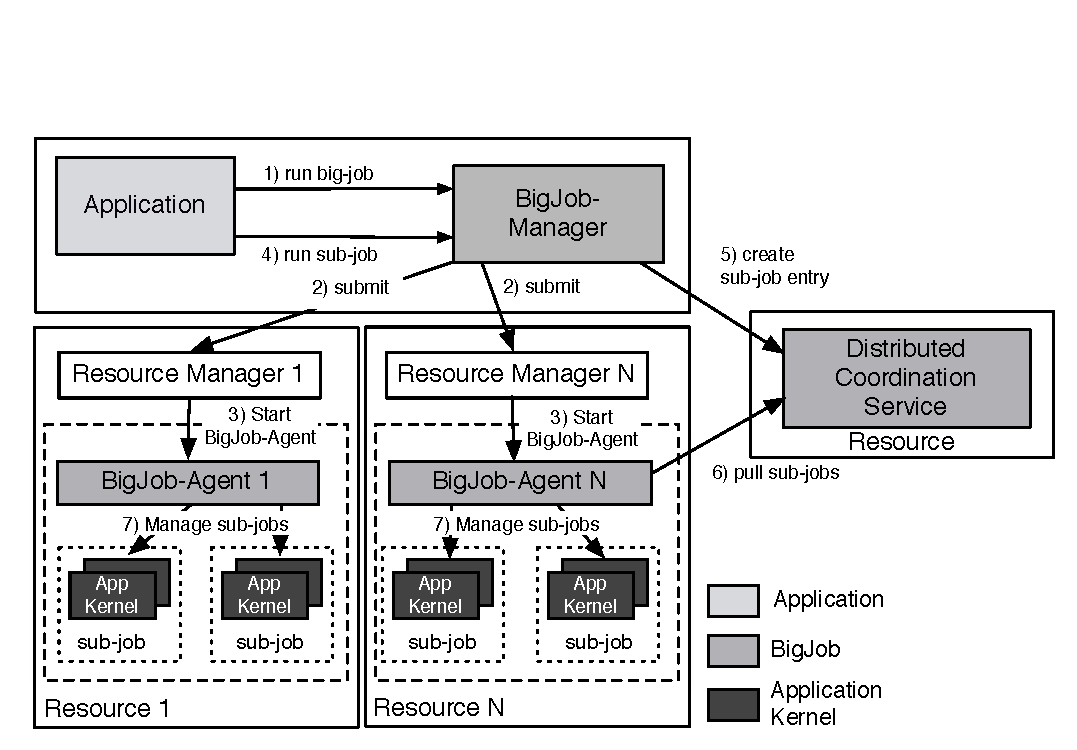
\includegraphics[width=0.7\textwidth]{figures/re_bigjob_interactions.pdf}
	\caption{\textbf{BigJob Architecture:} The
	          BJ architecture resembles many elements of the P* Model. The
	          BigJob-Manager is the central Pilot-Manager, which
	          orchestrates a set of Pilots. Each Pilot is represented by a
	          decentral component referred to as the BigJob-Agent.}
			\label{fig:figures_re_bigjob_interactions}
\end{figure}

Figure~\ref{fig:figures_re_bigjob_interactions} illustrates the BJ
architecture: The BJ-Manager is the Pilot-Manager responsible for coordinating
the different components of the frameworks. The BigJob-Agent is the actual
Pilot that is submitted to a resource. BigData extends the Pilot-Job concept
to data. BigData provides late-binding capabilities for data by separating the
storage allocation and application-level~\cite{pstar-2012}. Similar to BigJob,
it is comprised of two components: the BD-Manager and the BD-Agents, which are
deployed on the physical resources.

\begin{figure}[t] 
\centering 
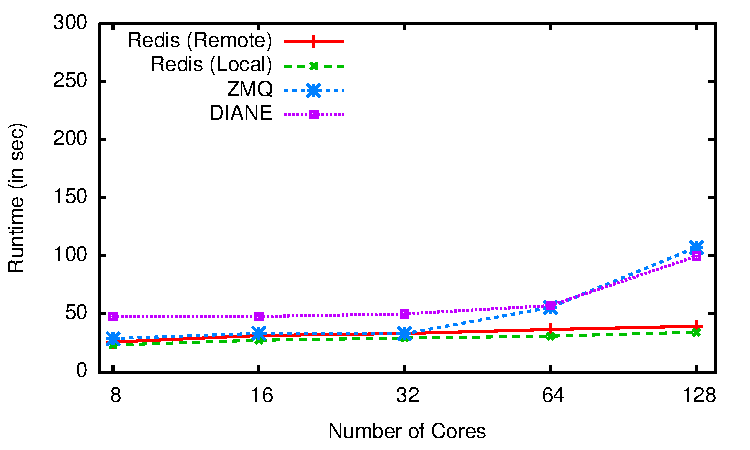
\includegraphics[width=0.8\textwidth]{figures/bigjob-varying-cores-alamo-noadvert.pdf}
\caption{\textbf{Pilot-Job Coordination Mechanism:}  The runtime of a
workload of 4 tasks per core, i.\,e.\ 32 - 512\,tasks, using different Pilots
and configuration. For BJ-Redis the runtime  increases only moderately, the
client-server-based implementations BJ-ZMQ and CORBA-based DIANE show
particularly a steep increase when going from 64 to 128 cores.}
\label{fig:perf_bigjob-varying-cores} 
\end{figure}

We used FutureGrid to evaluate the overheads typical associated with PJ
frameworks. For the evaluation of the communication \& coordination (c\&c)
subsystem of BigJob and DIANE we run a different number of very short running
(i.\,e. zero workload) tasks on Alamo/FG concurrently. In general, the c\&c
systems used are mostly insensitive to the number of coordinated tasks.

Figure~\ref{fig:perf_bigjob-varying-cores} illustrates the scalability of BJ
and DIANE with respect to the number of cores and tasks managed by Pilot. For
this purpose, we execute 4\,tasks per core, i.\,e.\ between 32 and 512\,tasks.
BigJob with Redis (local) shows almost linear scaling up to 128 cores. BigJob
with Redis (remote) imposes an increase of about 14\,\%. BigJob with ZeroMQ
performs very well with lower core counts; with larger core counts, the
runtimes increase, indicating a potential scalability bottleneck. Due to
higher startup overhead, at lower core counts DIANE shows a longer runtime
than ZeroMQ or Redis. At higher core counts DIANE behaves similar to
BigJob/ZeroMQ, but shows a greater increase in the overall runtime. This
increase is likely attributable to the single central manager in DIANE's
CORBA-based client-server architecture. Using Redis as central data space for
BigJob decouples Pilot-Manager and Agent, yielding better performance in
particular with many replicas.



% \section{Replica Exchange}
% 
% Various applications have been developed using Pilot Abstractions and BigJob.
% An important application class are those based on the Replica-Exchange
% algorithm. Replica-Exchange (RE) are used to understand physical phenomena –
% ranging from protein folding dynamics to binding affinity calculations. RE
% methods represent a class of algorithms that involve a large number of
% loosely-coupled ensembles. We develop a framework for RE that supports
% different replica-pairing and coordination mechanisms, that can utilize a
% range of production cyberinfrastructure concurrently. We use this framework to
% implement three different formulations of the RE algorithm: the synchronous, 
% asynchronous (centralized) and asynchronous (decentralized) formulation.
% 
% \alnote{Main issue: In Async-RE paper we only have TG/LONI numbers}
% \jhanote{I'm glad for RE to be removed from this paper and left as
%   Sai's contribution in the students paper. He has some graphs for
%   that too}

\section{Standards-based Interoperability}
\label{sec:standards}

There are two major approaches to allow applications to interoperably
use DCIs: system level interoperability (SLI) and application level
interoperability (ALI)~\cite{fgcs-interop11}.  SLI is the (often
standards based) approach to federate multiple DCIs on middleware and
operational level, and to allow applications to use the combined set
of resources as if it were a single DCI.  That implies the exchange of
accounting, authorization, authentication, logging, brokering and
resource management information, and others, on system level.  Very
often, SLI is implemented as delegation from one DCI to the other.

ALI on the other hand does not require any activity on infrastructure
level at all, but instead relies on the ability of the application to
utilize multiple independent DCIs at the same time.  While ALI is
usually easier to achieve, it typical increases the burden on the
application layer with the task to abstract the differences between
DCIs.

% Further, ALI based systems are inherently less sophisticated
%  and less complete than SLI based systems -- for example, data
%  transfer across DCI boundaries will need to be routed via the
%  application layer, accounting can't be managed on application layer
%  at all, etc. 

On real-world infrastructures, we usually encounter a need for both
approaches: while system-level standardization has found
uptake on % made tremendous
% steps toward system level interoperability for
a variety of
infrastructures (for example, BES is available on XSEDE, FutureGrid,
EGI, NorduGrid, Naregi and others), the level of SLI varies widely and
is often not the default modus operandi (BES again is not, as of yet,
the default interface on XSEDE and FutureGrid, and thus not available
on all resources).

As interoperability is a driving motivator behind the P* research
efforts described in the previous sections, we see the ultimate need
for application level interoperability, to complement SLI.  % At an
% architecture and implementation level, we largely base ALI on the
% 'Simple API for Grid Applications' (SAGA~\cite{ogf-gfd-90}), which we
% use as generic abstraction layer toward the distributed
% infrastructures. 
We use SAGA~\cite{ogf-gfd-90} to interface to a wide set of other
standards based backends (such as GridFTP, BES, DRMAA), but also
non-standards based ones (such as EC2/AWS/Eucalyptus, Condor,
Globus/GRAM) -- and thus utilizes SLI where available.

FutureGrid has been used in several critical aspects of the
standards-based approach.
First, we use FutureGrid as testing ground for standards
development\jhanote{Andre, I don't undertand what you mean by
  standards development. Sorry},
and for associated interoperability experiments on both the SLI and
ALI layer (see sec.~\ref{ssec:std_gin}).  Secondly, we use a variety
of backends provided by FutureGrid for developing SAGA as the
standards based access layer for our application level experiments (see
sec.~\ref{ssec:std_saga}).  And finally, we use FutureGrid in its
capacity as XSEDE targeted test environment to prepare and harden our
software, and its related packaging and deployment procedures, towards
enrolment on XSEDE, and on other infrastructures such as EGI (see
sec.~\ref{ssec:std_xsede}).

\subsection*{Standardization and OGF Interop Activities}
\label{ssec:std_gin}

 Standardization of interfaces and protocols is a crucial component
 for interoperability, even more so for SLI than for ALI.  For the
 target infrastructures of our research efforts (XSEDE, EGI, Naregi,
 OSG, FutureGrid), OGF related standards like BES, JSDL, GLUE, OCCI
 and SAGA are very relevant, but are largely still evolving and are
 still implemented and deployed.  The OGF Community Group 'GIN' (Grid
 Interoperation Now) is, for the scope of OGF, the umbrella group to
 host and coordinate efforts for interop testing and deployment.
 Resources on FutureGrid have been used both to develop and harden
 standard implementations as Genesis, Unicore and (from our end) SAGA,
 and also to test and demonstrate the SLI and ALI capabilities across
 those implementations, across a wide set of infrastructures.

 Within the scope of OGF, we have been showing a proof-of-concept
 distributed application (master-worker pattern, computing the
 Mandelbrot set -- see fig.~\ref{fig:mandelbrot}), which is able to
 concurrently utilize more than 30 systems distributed world-wide,
 which run $>$10 different middleware stacks, for a single application
 instance.  On FutureGrid alone, we have been using $>$10 submission
 endpoints on 4 different stacks for those experiments.  FutureGrid's
 capacity as research environment is greatly supporting that type of
 endeavour.

\begin{figure}[ht!]
 \begin{center}
  \subfigure[overview over participating backend states.]{
   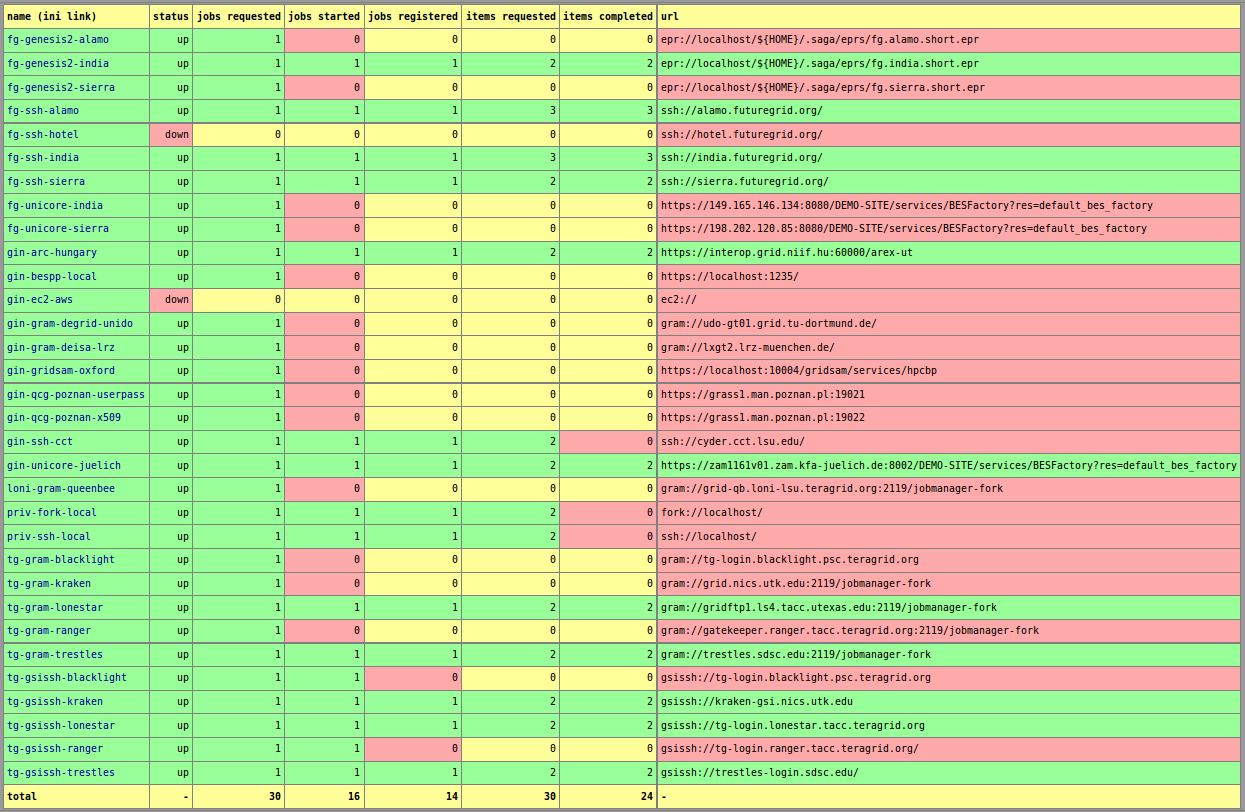
\includegraphics[width=0.48\textwidth]{figures/mandelbrot-table.png}
  }
  \subfigure[resulting mandelbrot set.]{
   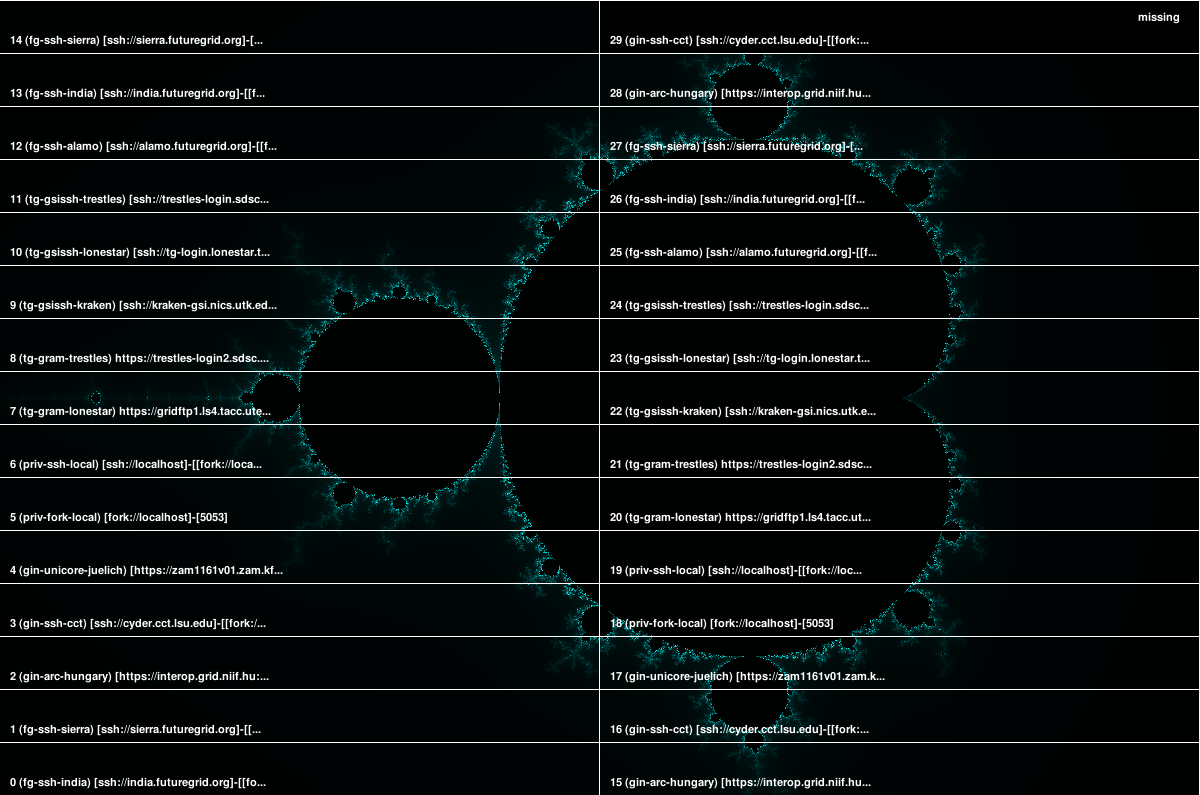
\includegraphics[width=0.48\textwidth]{figures/mandelbrot.png}
  }\vspace*{-1em}
  \caption{\textbf{Distributed Mandelbrot Demo}: the endpoints
   listed in table (a) contribute to the resulting mandelbrot set in
   figure (b).  Shown is an experimental snapshot which shows a number
   of endpoints in various error and success states.}
  \label{fig:mandelbrot}
 \end{center}
\end{figure}

 It must be noted that the greatest inhibitor of production level
 application runs on that scale is, at this point, not the
 engineering level -- a combination of ALI and SLI is well able to
 overcome most of the technical obstacles.  Instead, the security
 policies and accounting limitations for these efforts are what makes
 these experiments a continuous, and fragile, challenge.


\subsection*{Development of SAGA as an interoperable DCI Access Layer}
\label{ssec:std_saga}

 The described P* research and implementation efforts, and also the
 underlying ALI efforts, are mostly based on SAGA as generic
 abstraction layer for programming distributed applications and
 frameworks.  Our SAGA implementations are adaptor-based, i.e. they
 expose a generic API towards the application layer, whose semantics
 is provided by a set of adaptors which translate the API calls to the
 lower level system's capabilities.  As with all adaptor based
 systems, such an implementation is only as useful and stable as its
 backend bindings.  In particular, code stability is major concern, as
 SAGA requires integration with several middleware stacks, which in
 turn are based on a wide set of technologies, and are inherently
 complex.

 FutureGrid has been used as a development and testing environment for
 SAGA, allowing to implement and harden a wide number of backend
 adaptors, in particular new ones for BES and EC2/AWS.  The current
 move of FutureGrid toward (newer) OpenStack deployments will allow us
 to expand those efforts towards OCCI.  At the same time, the early
 availability of these backend bindings in SAGA has enabled several
 students and researchers to perform experiments on FutureGrid systems
 which would have been harder to achieve otherwise, thus increasing
 the usefulness of FutureGrid to its users.  Finally, the results of
 the SAGA implementation efforts are immediately usable for education
 and training efforts on FG, as described in~\ref{sec:edu}.


\subsection*{Providing Interoperability for Distributed Cyber Infrastructures}
\label{ssec:std_xsede}

 Next to the implementation challenges for ALI oriented system stand
 the deployment challenges.  In our experience, the efforts
 required to provide clean and stable deployment processes for
 a variety of environments can in fact well exceed the actual development
 efforts.

 We find the FutureGrid approach, to act as an test and staging
 environment which explicitly targets a large production environment,
 XSEDE, as very appropriate: it provides us with the ability to
 develop, test and certify packaging and deployment procedures without
 interfering with production systems, and without exposing the
 evolution of that process to the end users on those systems.  

 In detail: SAGA is deployed as community software on TeraGrid/XSEDE.
 We are using the same model on FutureGrid -- that provides SAGA
 installations to our (mostly experiment friendly) users on FutureGrid
 itself, and also perfectly mimics the procedures we use to deploy
 stable versions on XSEDE.  Further, we have been using FutureGrid
 resources to perform certification and packaging processes toward
 other production infrastructures, most notably toward the SAGA
 enrolment in the European EGI software repositories (UMD).


\section{Education: Distributed Scientific Computing}
\label{sec:edu}

In Fall of 2010 a new class on Scientific Computing was co-introduced
by Jha (led by Prof. Gabrielle Allen). The Distributed Scientific
Computing component of this class was led and developed by Jha.  The
module (Fig.~\ref{dsc}) covered the theory and practice of Distributed
Scientific Computing, with an emphasis on production-grade distributed
cyberinfrastructure.

There exist a broad range of computational infrastructure with varying
support for application characteristics, usage modes and even access
policies, all of which influence the usefulness of a given
infrastructure for scientific applications.  This module provided
sufficient understanding of production grade distributed
cyberinfrastructure to enable students to discern and determine which
infrastructure would be appropriate and effective for their
applications.

The module began by motivating the role and need for distributed
computing by understanding six rather different distributed
applications -- and analyzing them for the following points: why
distributed, how distributed and the challenges, success and/or issues
in distributing them. Elements of data-intensive computing and the
role of distributed data were also covered.  After establishing the
{\it essential} role of distributed computing in these applications,
as well as understanding the critical role of {\it execution
  environments} for distributed computing, the students were exposed
to a range of production distributed infrastructures and a brief
overview of the design principles, objectives and application
characteristics supported.  Specific examples of production Grids --
high-throughput as well as high-performance were analyzed.

To appreciate the reasons behind the rise of Cloud Computing, the
module provided a basic overview of the important underlying trend in
computing technology and data-intensive computing. This led to the
broader domain of scientific computing as enabled on commercial
infrastructure (Amazon EC2, Azure) as well as other non-commercial
Cloud offerings

%Clouds emerging infrastructure (eg Amazon EC2, Azure).  
 
Practically, the students were given hands on experience with both
virtualized resource and ``bare-metal'' resources thanks to the
FutureGrid. Students mostly experimented with Eucalyptus on India and
Sierra resources of the FutureGrid, as well as worked with a
SAGA-enabled version of MapReduce.

\begin{figure}[ht]
\centerline{
{\small
\begin{tabular}{|p{0.5cm}|p{3.5cm}|p{11.2cm}|}
\hline
& Lecture & Learning Objectives \\
\hline \hline
  E1 & Introduction to the Practise of Distributed Computing - I& WLCG as a motivating example (order of
  magnitude estimates of number of jobs submitted, data transferred,
  CPU cycles consumed), Distributed Application Exemplars, Analyzing
  why and how distributed, and challenges \& success in distribution.
   Introduction to SAGA and FutureGrid (FG). \\
  \hline
  E2 & Introduction to the Practise of Distributed Computing - II & Examples of Production Grid
  Infrastructure - HPC vs HTC, Research vs Production, Commercial.  Introduction to SAGA; Writing {\it your} first Dist.\ Application.  \\
  \hline
  E3 & Cloud Computing \& &  Cloud Computing. Convergence of
  multiple trends, Understanding Amazon \\
  & Master-Worker Pattern  & Examples of M-W Pattern: SAGA-based
  MapReduce, Word Count Application and Mandelbrot Set.\\
  \hline
  E4 & To Distributed or not to Distribute? & 
  Case Studies, Observations on Distributed Applications, Development
  Objectives; Projects on FG. \\
  \hline
\end{tabular}
}
}
\caption{\label{dsc} Module curricula for Distributed Scientific Computing} 
\end{figure}

The Sapir-Whorf hypothesis implies that ``language influences the
(habitual) thought''. The implication and analog in scientific
computing is that the infrastructure used shapes the
practise and formulation of research. Conversely, ``for a given
scientific application/research question, which cyberinfrastructure
should I use?''. Lecture E2  provided a brief overview and
understanding of available infrastructures, and E4 covered
the reasons and answers behind which infrastructure would be suitable
for a broad range of applications.


\section{Conclusion}


\bibliographystyle{plain}
\bibliography{pilotjob,saga,saga-related}


\end{document}
